% !TEX root = twe2.tex

\section{Diskussion}
\label{sec:Disukussion}
\textcite[33-36]{weggler2050leguminosen} hat Möglichkeiten zur Steigerung der \ac{NEL}-Erträge im Grünland Mithilfe von Rot- und Weißlklee untersucht.
Obwohl die \ac{NEL}-Erträge gesteigert werden konnten, sanken die \ac{NEL}-Gehalte (siehe \cref{subsec:NEL}).
\textcite{fritz2018wirtschaftliche} haben gezeigt, dass die Ernteverluste bei modernen Ernteverfahren bei etwa 20\% liegen.

%, allerdings ist zu beachten, dass aktuelle Verfahren der Futterkonxerierung zu hohen Verlusten führen, siehe \cref{subsec:Lit:Ernte}.
%Mit zukünftigen Ernte- und Konservierungsverfahren werden Landwirte hoffentlich Möglichkeiten haben die Verluste zu reduzieren.

\subsection{Literaturkritik}
\label{sub:kritik}

\begin{figure}
	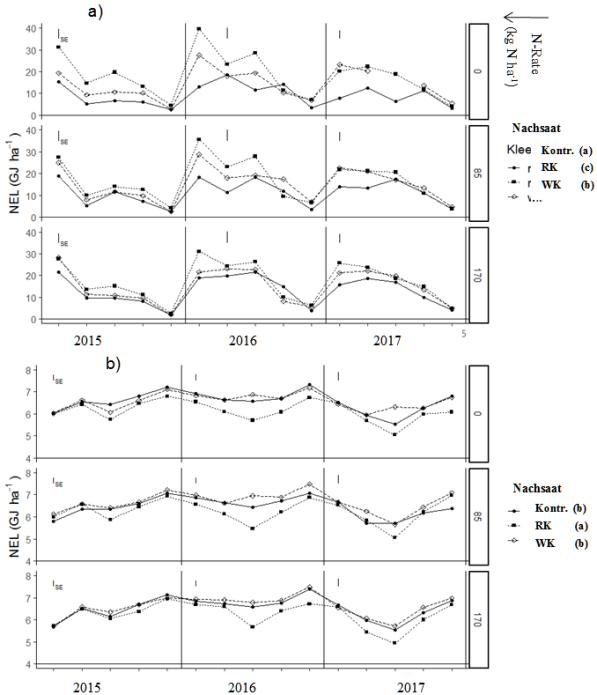
\includegraphics[scale=0.75]{images/wegglerAbb1}
	\caption[(a) \acs{NEL}-Ertrag und (b) \acs{NEL}-Konzentration in Abhängigkeit von der N-Düngung und Leguminosen Nachsaat über 3 Jahre]{(a) \ac{NEL}-Ertrag und (b) \ac{NEL}-Konzentration in Abhängigkeit von der N-Düngung und Leguminosen Nachsaat über 3 Jahre \parencite[35]{weggler2050leguminosen}}
	\label{fig:wegglerAbb1}
\end{figure}

In dem Arikel \parencite[33-36]{weggler2050leguminosen}\todo{Seitenangabe notwendig wenn die komplette Arbeit referenziert wird?} sind einige kleinere handwerkliche Fehler enthalten.
Das Thema \ac{NEL}-Ertragssteigerung über die Nachsaat von Klee in Grünlandbeständen wurde bisher wissenschaftlich kaum betrachtet (siehe \cref{subsec:NEL}).
Die Arbeit von \textcite{weggler2050leguminosen} richtet sich eindeutig an die aktuelle Forschung.
Die Veröffentlichung erfolgte im Zuge der 63. Jahrestagung der \ac{AGGF} auf welcher sich Wissenschaftler über die Zukunft des Grünlandes ausgetauscht haben.

Aufgrund der begrenzten Länge in dem Tagungsband erfolgt die Darstellugn der Daten, wie in wissenschaftlichen Veröffentlichungen üblich, sehr kompakt und auf das wichtigste reduziert.
Für Wissenschaftler, welche das Fachgebiet kennen, sind solche Einschränkungen kein Problem.
Allerdings ist es insbesondere für Landwirte kaum möglich, die Ergebnisse korrekt zu interpretieren.

In \textcite[35]{weggler2050leguminosen} ist die Legende sowie Achsbeschriftung, siehe \cref{fig:wegglerAbb1}, nicht korrekt umgesetzt.
%\todo{Numerierung ok? Verwendung Abk ok?, Breite ok? Müssen Abb. linksbündig sein?}
So wird zum Beispiel der \ac{NEL}-Gehalt mit GJ\,ha\textsuperscript{-1} beschrfitet, statt MJ\,kg\textsuperscript{-1} \ac{TM}.

Desweiteren wird die Abkürzung \ac{NEL} in der Einleitung nicht als \acl{NEL} eingeführt sondern als \textit{nutzbare Energie Laktation}.\todo{kursiv okay zum makieren von Fehlern?}
Im Kapitel Material und Methoden wird \ac{NEL} als \textit{Netto Energie Lactaion} bezeichnet.
In Abbildungsunterschriften wird widerholt \textit{nutzbare Energie Laktation} verwendet.
Normalerweise wird im landwirtschaftlichen Kontext die Abkürzung \acs{NEL} für \acl{NEL} verwendet.
Desweiteren ist \ac{NEL} eine wichtige Kenngröße in der Grundfuttermittelproduktion der Milchviehhaltung und somit der Grünlandwirtschaft.
Daher liegt es nahe einen Fehler in der Bezeichnung zu vermuten.

%Die Darstellung der \cref{fig:wegglerAbb1} ist nicht ideal.
%Die verschiedenen Messpunkte beziehen sich auf die einzelnen Aufwüchse, diese per Linie miteinander zu verbinden hilft zwar beim erkennen welcher Punkt zu welcher Datenreihe gehört, aber die Messdaten haben nicht die Aufgabe.
%Es gitb aber keine Datenpunkte welche zwischen den einzelnen Aufwüchsen liegt, welche man eventuell interpolieren könnte.
%Wen die x-Achse die N-Düngung angeben würde und die verschiedenen Schnitte in mehrere Diagramme aufgeteil worden wären, wobei bei jedem Schnitt jeweils der Durchschnitt der 3 Jahre genommen wird, wäre die Darstellung leichter verständlich.





\subsection{Sinnhaftigkeit einer Leguminosennachsaat}
\label{sub:leguminosen}
Wie in \cref{subsec:Protein} gezeigt, können Leguminosen den \ac{XP}-Ertrag vom Grünland erhöhen.
Der Versuch von \textcite{weggler2050leguminosen} wurde allerdings nur bis zu einer Düngung von 170\,kg\,N\,ha\textsuperscript{-1}a\textsuperscript{-1} gesteigert.
Daher ist es schwierig, einen Vergleich zwischen einer, in Norddeutschland üblichen,\todo{Zitat einfügen} N-Düngung von über 200\,kg\,N\,ha\textsuperscript{-1} sowie einer minimierten N-Düngung mit Leguminosen zu ziehen.
Eine Nachsaat mit Rotklee hatte häufig einen negativen Einfluss auf den \ac{XP}-Gehalt des Aufwuchs, während eine Weißlkleenachsaat tendenziell eine leichte Steigerung der \ac{XP} Gehalte zur Folge hatte.
Wie in \cref{subsub:alternative} gezeigt wird, ist der \ac{NEL}- und \ac{XP}-Gehalt eine sehr wichtige Größe in der Milchkughaltung. 
Generell sind deutliche Steigerungen des \ac{NEL}-Ertrages möglich, insbesondere bei (sehr) geringer N-Düngung, wobei insbesondere der Rotklee (siehe \cref{subsec:TM}) die \ac{TM} Erträge deutlich steigert.

Da der Rotklee zu einer signifikanten Verringerung der \ac{NEL}-Konzentration des Aufwuches geführt hat, ist für Milchviehbetriebe nachteilig.
Daher scheint eine Strategie mit einer Rot- und Weißklee Mischung als Nachsaat für die meisten Betriebe eine Option zu sein.
Bei Betrieben, welche eine etwas geringere Viehbesatzdichte haben, kann eine Weißkleenachsaat sinnvoller sein, da in diesem Fall geringere \ac{TM}-Erträge nicht so stark ins Gewicht fallen.
In weiteren Forschungen können die betriebswirtschaftlichen Einflüsse auf die Betriebe ausgearbeitet werden um den Beratern von milchviehhaltenden Betrieben eine wissenscahftlich fundierte Empfehlung geben zu können.

\subsubsection{Nährstoffkreislauf}
\label{subsub:nährstoffkreislauf}

In der Milchkuhhaltung besteht, wie in \cref{subsec:Stickstoff} gezeigt, ein Nährstoffkreislauf.
Dabei ist eine sehr große N-Quelle das Kraftfutter und über das Milcheiweiß verlässt ein Teil des Stickstoffs \todo{hier ausschreiben richtig?} den Betrieb.
%Über den Verkauf von Milch verlassen Nährstoffe, insbesondere N in Form des Milcheiweißes, den Betrieb.
%Falls der Betrieb den Wirtschaftsdünger abgibt, bzw. abgeben muss, verlassen darüber weitere Nährstoffe den Betrieb, unter anderem N.
%Nährstoffeinträge sind insbesondere über den Zukauf von Kraftfutter sowie, in eher geringen Mengen, der Einsatz von mineralischen Düngemitteln.
%Der Einsatz von Kraftfuttern ist für eine Milchkuh zur Steigerung der Milchleistung sehr sinnvoll.
%Eine Redufzierung des Kraftuffters ist, in den meisten Fällen, unwirtschaftlich.

Bei einer Reduzierung der N-Düngung auf den betriebseigenen Grünlandflächen ist, in den meisten Fällen, nicht mehr genügend Fläche vorhanden, um die eigenen Wirtschaftsdünger innerhalb des Betriebes zu verwerten.
Aufgrund der hohen Transportkosten ist eine Vewertung im nahem Umkreis anzustreben.
Insbesondere in Regionen mit einer hohen Besatzdichte an Milchkühen entsteht somit ein Überschuss an Wirtschaftsdüngern welcher exportiert werden muss.
Dies ist für die dort angesiedelten Betriebe eine große wirtschaftliche Herausforderung.
Nicht nur aufgrund der Transportkosten, welche in der Regel der abgebende Betrieb tragen muss, sondern auch, weil auch anderen Nährstoffe abgebeben werden und somit wieder zugekauft werden müssen.

Das von \textcite[33]{weggler2050leguminosen} angebrachte Argument, dass der Kraftfuttereinkauf gesellschaftlich kritisch gesehen wird und gesenkt werden sollte, muss umgesetzt werden, damit die Leguminosennachsaat sinnvoll wird.
Nur wenn weniger Stickstoff über das Kraftfutter in den Nährstoffkreislauf eingetragen wird, ist ein Stickstoffeintrag über Leguminosen sinnvoll.

\subsubsection{Leguminosen als alternative zu Kraftfutter}
\label{subsub:alternative}
Bei einem Einsatz von Leguminosen in der Grundfuttergewinnung ist, wie in \cref{subsec:NEL} gezeigt, eine Steigerung der \ac{NEL}-Erträge möglich.
Eine Reduzierung der Kraftfuttergabe ist, zumindestens für die meisten Betriebe mit intensiver Milchkuhwirtschaft, aufgrund der deutlich geringeren Milchleistung der Milchkühe nicht wirtschaftlich.
Für die Milchleistung ist der \ac{NEL}-Gehalt der Ration ein sehr wichtiger Parameter welcher über das Kraftuffter deutlich erhöht wird.
%Über das Kraftfutter wird kein Raufutter substituiert, daher ist der Einsatz von Kraftuffter unabhängig von der Qualität des Raufutters zu bewerten.

Falls die Kraftfutterkosten so weit steigen, dass dieses nurnoch eingesetzt werden, um eine ausgeglichene Ration zu erstellen, dann würde eine große N-Quelle für die Milchviehhaltung verloren gehen.
%, kann es sein, dass der Einsatz nicht mehr wirtschaftlich sinnvoll ist.
Eine andere Möglichkeit wäre, dass die \ac{EU} z.B. den Kraftfuttereinsatz in der Wiederkäuerfütterung einschränken könnte.
Da insbesondere Soja aus Südamerika, eine der wichtigsten \ac{XP}-Quellen der Milchkuhhaltung, gesellschaftlich in der Kritik steht, kann es passieren, dass die \ac{EU} entsprechende Schritte unternimmt.

Für den Fall dass der Eintrag von N über das Kraftfutter in den Nährstoffkreislauf deutlich reduziert wird, ändern sich die Vorraussetzungen.
Da der Verlust über den Verkauf von Milch bestehen bleibt, müssen neue Quellen erschlossen werden.
Eine Möglichkeit ist der Einsatz von mineralischen N-Düngemitteln, eine andere Möglichkeit wäre der Einsatz von Leguminosen.
In diesem Fall, je nach Entwicklung der Preise und bessierend auf den Ergebnissen von \textcite[33-36]{weggler2050leguminosen}, könnte eine Leguminosennachsaat kostengünstgier sein.


\subsection{Effizienz der Konservierung}
\label{sub:konservierung}
\ac{NEL}-Verluste während der Ernte, Konservierung oder Lagerung sind besonders kritisch zu betrachten.
Nachdem der Landwirt aufwändig hochwertiges Futter erzeugt hat, verliert dieses etwa 20\% des \ac{NEL}-Ertrags.
Diese Verluste sind aus betriebswirtschaftlicher Sicht langfristig nicht zu rechtfertigen.
Die Reduzierung dieser Verluste wird immer wichtiger, da vermutlich größere Anteile der \ac{NEL} über das Grundfutter abgedeckt werden muss.
Eine Verbesserung der Ernteverfahren bzw. Konservierungsmethoden ist daher dringend geboten.
Es bleibt somit zu hoffen dass die Forschung neue wirtschaftliche Verfahren entwickelt welche eine wirtschaftliche Nutzung des kompletten \ac{NEL}-Ertrags von landwirtschaftlichen Flächen erlaubt.

\subsection{Fazit}
\label{subsec:fazit}
Leguminosen sind eine sinnvolle Variante um die \ac{NEL}-Erträge des Grünlandes zu steigern.
Neben der Steigerung der Erträge wäre eine effizientere Verwertung dieser wünschenswert.
